\begin{figure}

\centering
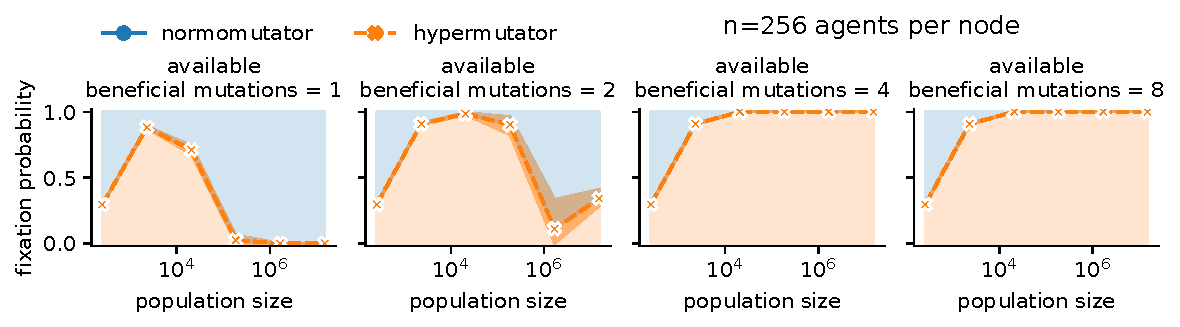
\includegraphics[width=0.8\linewidth]{binder/binder-wse-5050-spatial2d-2048atile-traits.ipynb/binder/teeplots/wse-5050-spatial2d-2048atile-traits/col=available-beneficial-mutations+errorbar=ci+hue=genotype+style=genotype+viz=size-fixation-areaplot+x=population-size+y=fixation-probability+ext=.pdf}%
\vspace{-3ex}
\caption{
\textbf{Restricted adaptive potential favors nonmutators.}
\footnotesize
Area plots show fixation probabilities in WSE simulations initialized with even mix of mutator and nonmutator genotypes.
As available beneficial mutations increase, mutattors gain favor in progressively larger populations.
% Simulations were conducted on WSE using the counter-based genome model, with populations initialized to a 50/50 mix of non- and mutators.
% Subpopulations comprised 2,048 agents per PE.
Shaded bands show bootstrapped 95\% confidence intervals.
% Supplementary Figure \ref{fig:fixheat-wse-altatile:2048} details results in a tabular format.
}
\label{fig:avail-ben-muts}

\vspace{-3ex}

\end{figure}


\section{Introduction} \label{sec:introduction}

% Mutation rates in microbial populations reflect a fundamental evolutionary trade-off.
While mutation is typically orders of magnitude more likely to harm fitness,
%, so low mutation rates increase the proportion of offspring that are viable.
in rare instances, mutation can introduce new beneficial traits.
% \citep{zeyl2004capturing,rozen2002fitness}.
Within asexual populations, such beneficial mutations can set into motion a winner-takes-all scenario where lineages unable to achieve comparable fitness gains are eventually driven to extinction.
% Hence, mutation can confer a rare --- but profound --- fitness benefit.

Like other phenotypic characteristics, the mutation rate of an organism can be strongly influenced by heritable traits --- for instance, by genes for DNA mismatch repair. %\citep{miller1998mutators}.
% Absent ongoing adaptive evolution, purifying selection will tend to suppress so-called ``mutator'' alleles.
In asexual populations lacking recombination, mutator alleles can  ``hitch-hike'' when a fitness-advantaged strain sweeps to fixation and carries along its full genetic background.
% In fact, as mutator alleles can systematically accelerate the pace of adaptive evolution \citep{orr2000rate}, they can even become evolutionarily favored due to generating linked beneficial alleles.
Understanding how and why mutator traits fix has broad importance in our understanding and management of evolving populations.
% Mutator traits have been shown to broadly influence the balance between selection and random effects on genetic content, profoundly accelerating processes of genetic drift \citep{couce2017mutator}.
% In particular, mutator strains can facilitate acquisition of novel pathogen traits such as antibiotic resistance, tumor progression, and changes in virulence.
% \citep{eliopoulos2003hypermutation,jolivetgougeon2011bacterial,stern2016viral,schlesner2015hypermutation,hammerstrom2015acinetobacter,perron2010hypermutability}.
For instance, the emergence of mutator strains has been associated with treatment using antibiotics of last resort \citep{mehta2019essential}.
% Spatial structure associated with biofilms, in particular, has been implicated in facilitating the evolution of antibiotic resistance \citep{france2018spatial}.
% Thus, beyond theoretical interest, studying mutator dynamics has concrete practical applications with real-world potential to benefit both individual health and public well-being.

Existing modeling work has established that large population size, in particular, can drive the probability of mutator traits fixing to near certainty \citep{raynes2018sign,tenaillon1999mutators}.
However, questions remain as to conditions that stabilize very large asexual populations \textit{against} mutator fixation \citep{raynes2019migration}.
Among other findings, reported work has allowed exploration of the role of mutational supply in curtailing mutator advantage in large populations (Figure \ref{fig:avail-ben-muts}), as well as the sensitivity of this effect to population structure and background rates of mutator allele prevalence.

% \subsection{Causes and Consequences of Mutator Strains}

% Mutator strains are observed across a wide variety of populations, including both natural systems and laboratory experiments \citep{sniegowski1997evolution,swings2017adaptive,maddamsetti2020divergent,cherry2018methylation,notleymcrobb2002enrichment,shaver2002fitness,voordeckers2015adaptation,leclerc1996high}.
% As such, a substantial body of literature has investigated the conditions under which mutator traits tend to arise.
% As mentioned above, population size has been implicated as a key factor for mutator fixation, as large populations provide more opportunities for the beneficial mutations that drive mutator hitch-hiking \citep{chao1983competition}.
% On the other hand, bottleneck events that suddenly reduce population size can suppress mutator fixation by disrupting propagation of the beneficial alleles that mutators hitchhike off of \citep{raynes2013effect}.

% A wide variety of computational and mathematical modeling approaches have been applied in studying the evolutionary dynamics of mutator alleles.
% Although tangential to the present work, mathematical and computational investigations have notably treated a broad variety of additional topics, including coevolutionary pressures \citep{pal2007coevolution} and interactions with sexual recombination \citep{johnson1999beneficial}.
% Within the purifying selection regime (i.e., absent positive selection for beneficial traits), modeling work has also investigated the interplay between mutator alleles and Muller's ratchet \citep{soderberg2011kickstarting} and dynamics steering towards evolutionarily stable mutation rates \citep{lynch2008cellular}.

% Of more direct salience to present work, \citet{desai2011balance} provide a key foundation in understanding transient fluctuations in mutator allele prevalence, who focus on a dynamic (rather than steady-state) framing of the topic.
% For scenarios with positive selection, attention is first paid to the probability for a given \textit{de novo} beneficial mutation to survive drift effects and reach sufficient frequency to be reliably selected upon.
% Principled approximations are applied to suggest parameter regimes where establishment probability for beneficial alleles arising on a mutator background may safely be considered to be essentially zero (i.e., mutator incurs catastrophic mutational load) and where establishment probability is essentially indistinguishable from nonmutators (i.e., mutator incurs negligible mutational load).
% At these extrema, mutator fixation probability is shown to follow easily from establishment probabilities under the condition that fixation time may be assumed sufficiently short to neglect the possibility of competition between more than one established allele.
% However, in scenarios where either (1) fixation times are long (e.g., large population size) or (2) the mutational load incurred by mutators falls within an intermediate parameter range, matters are noted to become substantially more involved.
% At this point, \citet{desai2011balance} conclude their analysis with a heuristic discussion outlining expected qualitative regimes within these remaining regions of parameter space.
% In line with themes explored in present work, \citet{desai2011balance} note that where fixation times for mutator alleles hitch-hiking with a given beneficial mutation are sufficiently long, establishment of a commensurate beneficial mutation among nonmutators prior to fixation becomes inevitable.
% Therefore, successive adaptive mutations become necessary in such cases to fix a mutator allele.

% Several earlier works provide further insight into the role of adaptive potential in the evolutionary dynamics of mutator alleles.
% The core dynamic by which successive adaptive mutations can ultimately fix a mutator allele is demonstrated by \citet{tanaka2003evolution}.
% Through a combination of analytical and computational modeling, they show how mutator alleles can rise in frequency over the course of a selective sweep for a single beneficial mutation, even if nonmutators are first to discover the beneficial mutation.
% Although beyond the scope of their analyses, it is noted that such an effect could compound over successive adaptive sweeps to boost mutator prevalence.
% Somewhat relatedly, \citet{travis2002mutator} apply a deterministic model to show that mutator concentration can creep progressively above baseline equilibrium when adaptive potential associated with environmental changes becomes available.
% Most pertinently, however, \citet{tenaillon1999mutators} directly demonstrate mutator ratcheting over successive sweeps in a set of extensive finite-sized stochastic simulations, which apply efficient compartment-based representations to model the genetic composition of large well-mixed populations.
% In their simulations, time series traces of mutator proliferation from background levels exhibit clear multistep dynamics.
% Of particular note, simulations using a fixed population size of $10^9$ demonstrate the fixation probability of mutators to increase with the number of adaptive mutations available.

% Recent \textit{in vivo} experimental work has established direct evidence for connections between adaptive potential and mutator outcomes.
% In this work, \citet{callens2023hypermutator} conducted treatments exposing populations of \textit{E. coli} to either antibiotic or osmotic stressors, calibrated to comparable severities.
% Because the antibiotic agent employed in experiments targeted a pathway involving relatively few genes, fewer loci exhibited adaptive potential compared to the large number of pathways implicated by the osmotic stress condition.
% In line with theoretical expectations, the high-adaptive-potential osmotic stressor induced significantly higher rates of mutator fixation.
% More broadly, existing work has drawn clear connections between elevated mutation rate and long-term environmental, coevolutionary, or ecological fluctuations that introduce a moving evolutionary target \citep{leigh1970natural,travis2002mutator,travis2004mutators,rosenbloom2014frequencydependent,pal2007coevolution,wei2022rapid}.

% In a separate vein of inquiry, work by \citet{raynes2018sign} is notable in establishing a systematic understanding of the impact of population size on mutator allele favorability.
% Through paired agent-based simulation and yeast-model experiments, a striking sign-change effect is demonstrated to play out along the spectrum of population size.
% A quantitative basis for this effect is provided by synthesizing independent analytical approximations for the probability of mutator fixation by drift and hitchhiking.
% For small population sizes, mutator alleles' selective cost of imposed deleterious load outweighs their selective benefit in facilitating the discovery of beneficial mutations.
% In larger population sizes, the relative magnitude of these effects switches and mutator alleles become favored via indirect selection for generated beneficial mutations.

% Earlier work has also pointed to the role of population size influencing selection on mutators.
% \citet{wylie2009fixation} apply stochastic simulation and diffusion-based analytical methods to study mutator dynamics in asexual populations, partly describing how large population size can favor mutators.
% A similar conclusion is reached by \citet{andre2006evolution}, through analytical models based in game theory.
% Work by \citet{good2016evolution}, notable for extending analytical modeling efforts into the parameter regime where clonal interference between competing beneficial mutations is at play, also predicts population size to increase fixation probability within well-mixed populations.
% This prediction is validated through forward-time Wright-Fisher simulations.
% (Other aspects of this work are notable in considering effects of mutator alleles on population-level adaptation rates and transient overshooting of evolutionarily stable mutation rates.)

% In this work, we seek to extend understanding of how limited adaptive potential interacts with population size and structure to influence mutator dynamics within asexual populations.
% As noted earlier, such knowledge is needed to improve explanation of how nonmutator alleles can be maintained within large populations.
% In \citep{raynes2018sign}, concluding remarks hypothesize that spatial structure may help to explain why mutator alleles do not universally fix within large asexual populations.
% However, in a later set of paired \textit{in vivo}/\textit{in vitro} experiments, deviation from well-mixed conditions is contradictorally linked to \textit{higher} probability for mutator fixation if any level connectivity remains between subpopulations \citep{raynes2019migration}.
% A simple explanation is provided for this result: although mutators are disfavored within the small population size of an isolated deme, a fixed mutator within any single deme will subsequently invade all remaining demes due to outcompeting nonmutator strains in accruing subsequent adaptive potential.
% Thus, long-term nonmutator persistence requires short-term mutator extinction within \textit{all} subpopulations, such mutator extinction becomes increasingly unlikely with high deme counts.
% In this work, we hypothesize that an opposite effect will occur where adaptive potential is limited.
% Under such a scenario, long-term nonmutator persistence requires short-term nonmutator survival within only a single subpopulation, which can successfully invade mutator subpopulations due to lower mutational load once available adaptive potential is exhausted.

% \subsection{Major Results}

% In our initial experiment, we confirmed that large populations favor mutator fixation, under the assumption of unlimited adaptive potential.
% Consistent with expectations, we found that restricting adaptive potential by capping available adaptive mutations reversed outcomes in large populations to favor nonmutators.
% Investigating the influence of population structure and composition, we found spatial structure to substantially increase the amount of adaptive potential required to fix mutator alleles in large populations.
% However, this effect only occurred when mutator alleles were initially rare within the population.
% We also report qualitative differences between effects of population size on mutator fixation probability under well-mixed versus 2D population structure when mutations are rare.
% In the final part of our investigation, we analyze the spatiotemporal dynamics of our simulations to better understand the mechanisms at play behind these effects.

% Differing from existing results, we find that in the situation of limited adaptive potential, the effect of population structure on fixation probability is actually opposite to that predicted under the theory.
% Population structure has also been found to influence mutator outcomes, with deviation from well-mixed conditions being linked to a higher probability for hypermutator fixation so long as any connectivity remains between subpopulations \citep{raynes2019migration}.

% Of technical note, the large-scale simulations necessary for this work were made possible by exploiting hardware accelerator platforms --- specialized high-performance computing (HPC) peripherals capable of massive computational workloads.
% In line with existing work applying Graphics Processing Units (GPUs) for agent-based modeling \citep{turpin2021xaevol,kosiachenko2019mass,perumalla2009switching,heinemann2007artificial,richmond2023flame}, we found a substantial performance boost: in our case, $378\times$ speedup over single-core CPU evaluation.
% \footnote{%
% Other notable approaches to large-scale evolution simulations have used more traditional cluster-based CPU modeling \citep{moreno2022best,collier2015large,ray1995proposal,turpin2020paevol}, sampling-based approximations \citep{taddei1997role}, and compartmental representations \citep{tenaillon1999mutators}.}
% We also leveraged Wafer-Scale Engine (WSE) technology in this work, a cutting-edge AI/ML-oriented platform that delivers 850,000 processor cores packed together on a single chip.
% Simulation on WSE achieved a further $294\times$ speedup, resulting in a net $111{,}091\times$ speedup from single-CPU evaluation.
% These performance gains ultimately benefited the work by allowing us to employ forward-time agent-based simulation at full resolution across genome models and population structures that are difficult to integrate with compartment-based approaches used for simulations of large populations in existing work.

% These performance gains ultimately benefited the work by allowing us to employ forward-time agent-based simulation at full resolution across genome models and population structures that are difficult to integrate with compartment-based approaches used for simulations of large populations in existing work.

To enable the simulation scale necessary for this work, we employed Graphics Processing Unit (GPU) and Wafer-Scale Engine (WSE) hardware accelerators.
The Cerebras CS-2 WSE, in particular, is notable among an emerging class of next-generation AI/ML-oriented hardware accelerators.% \citep{lauterbach2021path}.
This chip comprises a grid lattice of 850,000 independent processor elements (PEs), networked for low-latency communication among neighboring PEs.
Explorations are ongoing in establishing applications of these platforms for scientific and high-performance computing (see e.g., \citep{rocki2020fast,ltaief2023scaling,sai2023massively}).

Notably, however, major challenges exist in adapting simulation codes to the WSE platform's dataflow paradigm and extreme constraints in memory use and communication locality.
At the hardware level, all communication occurs through message passing between directly adjacent processing tiles.
Additionally, although on-device memory totals 40GB, only 48kb is available per PE.
We address these constraints by mapping WSE layout to simulation spatial structure and adopting dynamic data coarsening strategies, discussed next.
In concert with traditional observational and experimental work, harnessing such next-generation hardware accelerator platforms promises to ultimately contribute in extending biological understanding across broader scales and levels of organization.
%The ability to leverage emerging HPC architectures, as shown here, offers a practical step toward addressing such challenges.


% A key trade-off encountered in this work is in memory constraints imposed by WSE architecture, which supplies only 48kb of memory per PE.

% Of technical note, the large-scale simulations necessary for this work were made possible by exploiting hardware accelerator platforms --- specialized high-performance computing (HPC) peripherals capable of massive computational workloads.
% In line with existing work applying Graphics Processing Units (GPUs) for agent-based modeling \citep{turpin2021xaevol,kosiachenko2019mass,perumalla2009switching,heinemann2007artificial,richmond2023flame}, we found a substantial performance boost: in our case, $378\times$ speedup over single-core CPU evaluation.
% \footnote{%
% Other notable approaches to large-scale evolution simulations have used more traditional cluster-based CPU modeling \citep{moreno2022best,collier2015large,ray1995proposal,turpin2020paevol}, sampling-based approximations \citep{taddei1997role}, and compartmental representations \citep{tenaillon1999mutators}.}
% We also leveraged Wafer-Scale Engine (WSE) technology in this work, a cutting-edge AI/ML-oriented platform that delivers 850,000 processor cores packed together on a single chip.
% Simulation on WSE achieved a further $294\times$ speedup, resulting in a net $111{,}091\times$ speedup from single-CPU evaluation.



% In the CORE of our experimental work, we sought to establish how adaptive potential interacts with current synthesis of the role of population size in mediating mutator dynamics.
% This involved conducting a series of trials across WSE,
% Due to the inherent spatial structure owing to local connectivity on the WSE, aspects of experiments were complimented by GPU to provide perspective under well-mixed conditions.

% At the core of these broader experiments is the finding

% Figure \ref{fig:avail-ben-muts} shows fixation curves where one, two, three, four, and five beneficial mutations are available, conducted with 256 agents per deme.
% Under surveyed conditions, with 2D spatial structure and mutators initially in equal proportion to nonmutators, nonmutator persistence rapidly decays with increases in adaptive potential.
% Even with the largest surveyed billion-agent population size, mutators regain selective parity where four or more beneficial mutations are available.

% One assumption of existing work by \citet{raynes2018sign} is availability of abundant potential beneficial mutations.
% Existing simulation studies suggest that restricting adaptive potential should disfavor mutator alleles \citep{tenaillon1999mutators}, but understanding of how this effect interacts with other factors is limited.

% To investigate this question, we performed experiments where the supply of possible beneficial mutations was constrained.
% Experiments were conducted on the WSE platform using 2D population structure with 50/50 initialization.
% The right panels of \cref{fig:wse-inf-one:32,fig:wse-inf-one:2048} show mutator fixation probabilities where agents could accrue no more than one beneficial mutation for trials using 32 and 2,048 agents per deme, respectively.
% In both cases, a second sign-change fitness effect for mutator traits appears, with nonmutators regaining favor past population sizes of 100,000 agents.
% Beyond population sizes of 1 million agents, nonmutators reliably drive mutators to extinction.

% These results substantiate an earlier verbal hypothesis by \citet{desai2011balance} that more than one beneficial mutation should become necessary to fix a mutator allele when fixation time becomes long, as is the case with large population size.
% The rationale behind this expectation is that where fixation time is long, non-mutators are more likely to discover a comparable beneficial allele before being driven to extinction.
% From this point, disadvantage in mutational load dooms the mutator allele.




% Next, we tested sensitivity of the relationship between mutator fixation probability and population size with respect to the amount of adaptive potential available.

% Interestingly, this result may help explain an earlier observation by \citet{tenaillon1999mutators} that below a threshold of four beneficial mutations available, mutator alleles never rose from background levels to fix within their compartment-based model of a well-mixed billion-member population.
% Notwithstanding differences in model parameterization and population structure, our findings suggest that this threshold may coincide with the point where the net fitness effect of the mutator allele neutralizes in commensurately scaled populations.
